% !TEX program = xelatex
\documentclass[12pt,a4paper]{article}

\usepackage{fontspec}
\usepackage{polyglossia}
\setmainlanguage{greek}
\setotherlanguage{english}
\setmainfont[Script=Greek]{DejaVu Serif}
\setsansfont[Script=Greek]{DejaVu Sans}
\setmonofont[Script=Greek]{DejaVu Sans Mono}
\newfontfamily\greekfonttt[Script=Greek]{DejaVu Sans Mono}

\usepackage[a4paper, margin=2.45cm]{geometry}
\usepackage{amsmath, amssymb}
\usepackage{booktabs}
\usepackage{array}
\usepackage{graphicx}
\usepackage{float}
\usepackage{caption}
\usepackage[hidelinks]{hyperref}
\usepackage{enumitem}
\usepackage{parskip}
\usepackage{xcolor}
\usepackage{listings}
\usepackage{fancyhdr}

\pagestyle{fancy}
\fancyhf{}
\lhead{4η Εργασία -- Explanatory Report}
\rhead{Ερώτημα 2}
\cfoot{\thepage}
\setlength{\headheight}{14.5pt}

\newcommand{\code}[1]{\texttt{\textenglish{#1}}}

\lstset{
    basicstyle=\ttfamily\small,
    breaklines=true,
    frame=single,
    backgroundcolor=\color{gray!8},
    columns=fullflexible,
    keepspaces=true
}

\title{
    \textbf{Ανάλυση Δεδομένων 2025--26}\\[0.25cm]
    \Large 4η Εργασία -- Explanatory Report\\[0.15cm]
    \large Ερώτημα 2: Bagging με 200 εκτιμητές
}
\author{
    Ρακοβαλής Παύλος\\
    ΑΕΜ: 6931
}
\date{\today}

\begin{document}

\maketitle
\thispagestyle{fancy}

\begin{abstract}
Το παρόν κείμενο είναι ένα αναλυτικό, επεξηγηματικό report για το δεύτερο
ερώτημα της 4ης εργασίας. Στόχος είναι να εξηγηθεί η μέθοδος Bagging με τρόπο
κατανοητό ακόμη και σε κάποιον που δεν έχει προηγούμενη εμπειρία στην Ανάλυση
Δεδομένων. Πρώτα παρουσιάζεται τι ζητάει το ερώτημα, στη συνέχεια εξηγείται
το θεωρητικό υπόβαθρο της μεθόδου και τέλος περιγράφεται βήμα προς βήμα η
υλοποίηση με 200 εκτιμητές. Το μοντέλο Bagging πέτυχε test accuracy 0.9660,
δηλαδή ταξινόμησε σωστά περίπου το 96.60\% των test παρατηρήσεων.
\end{abstract}

\tableofcontents
\newpage

%=============================================================================
\section{Το ερώτημα της εργασίας}
%=============================================================================

Το δεύτερο ερώτημα της 4ης εργασίας είναι:

\begin{quote}
\textbf{«Να γίνει πρόβλεψη/εκτίμηση του τύπου κρασιού με τη μέθοδο Bagging,
χρησιμοποιώντας εκτιμήσεις από 200 δειγματοληψίες
(\code{n\_estimators=200}).»}
\end{quote}

Με απλά λόγια, η εργασία ζητάει να προβλέψουμε αν ένα κρασί είναι λευκό ή
κόκκινο, όπως και στο πρώτο ερώτημα. Η διαφορά είναι ότι τώρα δεν θα
χρησιμοποιήσουμε μόνο ένα δέντρο ταξινόμησης. Θα χρησιμοποιήσουμε πολλά
δέντρα μαζί.

Η μέθοδος Bagging λειτουργεί ως εξής:

\begin{itemize}
    \item δημιουργεί πολλά διαφορετικά δείγματα από το training set,
    \item εκπαιδεύει ένα δέντρο ταξινόμησης σε κάθε δείγμα,
    \item παίρνει την πρόβλεψη κάθε δέντρου,
    \item και στο τέλος αποφασίζει με ψηφοφορία.
\end{itemize}

Στο συγκεκριμένο ερώτημα ο αριθμός των δέντρων είναι:

\begin{center}
\code{n\_estimators = 200}
\end{center}

Δηλαδή το μοντέλο δεν στηρίζεται σε μία μόνο γνώμη, αλλά σε 200 διαφορετικά
δέντρα ταξινόμησης.

\subsection{Τι ακριβώς πρέπει να παραδώσουμε}

Για να λυθεί πλήρως το δεύτερο ερώτημα, πρέπει να γίνουν τα εξής:

\begin{enumerate}[label=\arabic*.]
    \item Να χρησιμοποιηθούν τα ίδια δεδομένα της 3ης εργασίας.
    \item Να χρησιμοποιηθεί ως στόχος η μεταβλητή \code{wine\_type}.
    \item Να εξαιρεθεί η μεταβλητή \code{quality}, όπως ζητάει η εκφώνηση.
    \item Να γίνει ο ίδιος διαχωρισμός σε training set 70\% και test set 30\%.
    \item Να εφαρμοστεί η μέθοδος Bagging με \code{n\_estimators=200}.
    \item Να γίνουν προβλέψεις στο test set.
    \item Να υπολογιστεί η test accuracy.
    \item Να παρουσιαστεί και να ερμηνευτεί ο confusion matrix.
\end{enumerate}

%=============================================================================
\section{Υπενθύμιση του προβλήματος}
%=============================================================================

Το πρόβλημα είναι πρόβλημα ταξινόμησης. Θέλουμε να πάρουμε τις φυσικοχημικές
μετρήσεις ενός κρασιού και να αποφασίσουμε αν είναι:

\begin{center}
\code{red} ή \code{white}.
\end{center}

Η μεταβλητή στόχος είναι:

\begin{center}
\code{wine\_type}.
\end{center}

Η κωδικοποίηση που χρησιμοποιήθηκε είναι:

\begin{center}
\code{red = 0} \hspace{1cm} και \hspace{1cm} \code{white = 1}.
\end{center}

Οι προβλεπτικές μεταβλητές είναι όλες οι υπόλοιπες φυσικοχημικές μεταβλητές,
εκτός από τη \code{quality}. Συνολικά χρησιμοποιούνται 11 predictors.

\begin{center}
\footnotesize
\begin{tabular}{lll}
\toprule
\code{fixed acidity} & \code{volatile acidity} & \code{citric acid} \\
\code{residual sugar} & \code{chlorides} & \code{free sulfur dioxide} \\
\code{total sulfur dioxide} & \code{density} & \code{pH} \\
\code{sulphates} & \code{alcohol} & \\
\bottomrule
\end{tabular}
\end{center}

\subsection{Το ίδιο train/test split με το Ερώτημα 1}

Για να είναι δίκαιη η σύγκριση με το προηγούμενο ερώτημα, χρησιμοποιήθηκε το
ίδιο train/test split:

\begin{center}
\begin{tabular}{lrr}
\toprule
\textbf{Σύνολο} & \textbf{Πλήθος} & \textbf{Ποσοστό} \\
\midrule
Training set & 3706 & 70\% \\
Test set & 1589 & 30\% \\
\bottomrule
\end{tabular}
\end{center}

Επίσης χρησιμοποιήθηκε:

\begin{center}
\code{random\_state = 6931}
\end{center}

και \code{stratify=y}, ώστε να διατηρηθεί παρόμοια αναλογία κόκκινων και
λευκών κρασιών στο training και στο test set.

%=============================================================================
\section{Θεωρητικό υπόβαθρο: γιατί δεν αρκεί πάντα ένα δέντρο}
%=============================================================================

Στο πρώτο ερώτημα χρησιμοποιήσαμε ένα δέντρο ταξινόμησης μέγιστου βάθους 2.
Το δέντρο αυτό είχε το πλεονέκτημα ότι ήταν απλό και εύκολα ερμηνεύσιμο.
Όμως ένα μόνο δέντρο έχει και ένα βασικό μειονέκτημα: μπορεί να είναι
ασταθές.

\subsection{Τι σημαίνει ότι ένα δέντρο είναι ασταθές}

Ένα δέντρο ταξινόμησης φτιάχνεται κάνοντας διαδοχικούς διαχωρισμούς στα
δεδομένα. Αν αλλάξουν λίγο τα training δεδομένα, μπορεί να αλλάξουν και οι
διαχωρισμοί που επιλέγει το δέντρο. Άρα μπορεί να καταλήξουμε σε διαφορετικό
δέντρο.

Με απλά λόγια:

\begin{quote}
Ένα δέντρο μπορεί να επηρεάζεται αρκετά από τις λεπτομέρειες του συγκεκριμένου
training set.
\end{quote}

Αυτό δεν σημαίνει ότι τα δέντρα είναι κακή μέθοδος. Σημαίνει όμως ότι ένα μόνο
δέντρο μπορεί να έχει σχετικά μεγάλη διακύμανση. Δηλαδή, αν εκπαιδευτεί σε
λίγο διαφορετικά δεδομένα, μπορεί να δώσει λίγο διαφορετικό μοντέλο.

\subsection{Η βασική ιδέα των ensemble μεθόδων}

Οι ensemble μέθοδοι προσπαθούν να βελτιώσουν την πρόβλεψη συνδυάζοντας πολλά
μοντέλα.

Η ιδέα είναι απλή:

\begin{quote}
Αν ένα μοντέλο μπορεί να κάνει λάθος, πολλά μοντέλα μαζί μπορεί να δώσουν πιο
σταθερή και πιο αξιόπιστη απόφαση.
\end{quote}

Αυτό μοιάζει με την ιδέα της ψηφοφορίας. Αν ρωτήσουμε μόνο ένα άτομο, μπορεί
να κάνει λάθος. Αν όμως ρωτήσουμε 200 άτομα και πάρουμε την πλειοψηφική
απάντηση, η τελική απόφαση μπορεί να είναι πιο σταθερή.

Το Bagging είναι μία από τις πιο βασικές ensemble μεθόδους.

%=============================================================================
\section{Θεωρητικό υπόβαθρο: τι είναι το Bagging}
%=============================================================================

Η λέξη Bagging προέρχεται από τη φράση:

\begin{center}
\textenglish{Bootstrap Aggregating}.
\end{center}

Η φράση αυτή έχει δύο κομμάτια:

\begin{itemize}
    \item \textbf{Bootstrap}: δημιουργούμε πολλά νέα δείγματα από το αρχικό
    training set.
    \item \textbf{Aggregating}: συνδυάζουμε τις προβλέψεις πολλών μοντέλων.
\end{itemize}

\subsection{Τι είναι bootstrap δείγμα}

Ένα bootstrap δείγμα είναι ένα δείγμα που φτιάχνεται από το training set με
δειγματοληψία \textbf{με επανάθεση}.

Η φράση «με επανάθεση» σημαίνει ότι κάθε φορά που επιλέγουμε μία παρατήρηση,
την ξαναβάζουμε πίσω στο σύνολο, άρα μπορεί να επιλεγεί ξανά.

Παράδειγμα:

\begin{quote}
Αν έχουμε τις παρατηρήσεις A, B, C, D, ένα bootstrap δείγμα μεγέθους 4 θα
μπορούσε να είναι A, C, C, D. Η παρατήρηση C εμφανίζεται δύο φορές, ενώ η B
δεν εμφανίζεται καθόλου.
\end{quote}

Στο Bagging δημιουργούνται πολλά τέτοια bootstrap δείγματα. Σε κάθε δείγμα
εκπαιδεύεται ένα μοντέλο.

\subsection{Τι σημαίνει n\_estimators}

Η παράμετρος \code{n\_estimators} δηλώνει πόσα επιμέρους μοντέλα θα
εκπαιδευτούν.

Στο ερώτημα αυτό:

\begin{center}
\code{n\_estimators = 200}
\end{center}

Άρα το Bagging δημιουργεί 200 bootstrap δείγματα και εκπαιδεύει 200 δέντρα
ταξινόμησης. Κάθε δέντρο δίνει τη δική του πρόβλεψη και στο τέλος οι
προβλέψεις συνδυάζονται.

\subsection{Πώς αποφασίζει τελικά το Bagging}

Επειδή έχουμε πρόβλημα ταξινόμησης, το Bagging χρησιμοποιεί πλειοψηφική
ψηφοφορία.

Για παράδειγμα, έστω ότι για ένα συγκεκριμένο κρασί:

\begin{itemize}[nosep]
    \item 170 δέντρα προβλέπουν \code{white},
    \item 30 δέντρα προβλέπουν \code{red}.
\end{itemize}

Τότε η τελική πρόβλεψη του Bagging είναι:

\begin{center}
\code{white}.
\end{center}

Δηλαδή το μοντέλο επιλέγει την κλάση που πήρε τις περισσότερες ψήφους.

\begin{figure}[H]
\centering
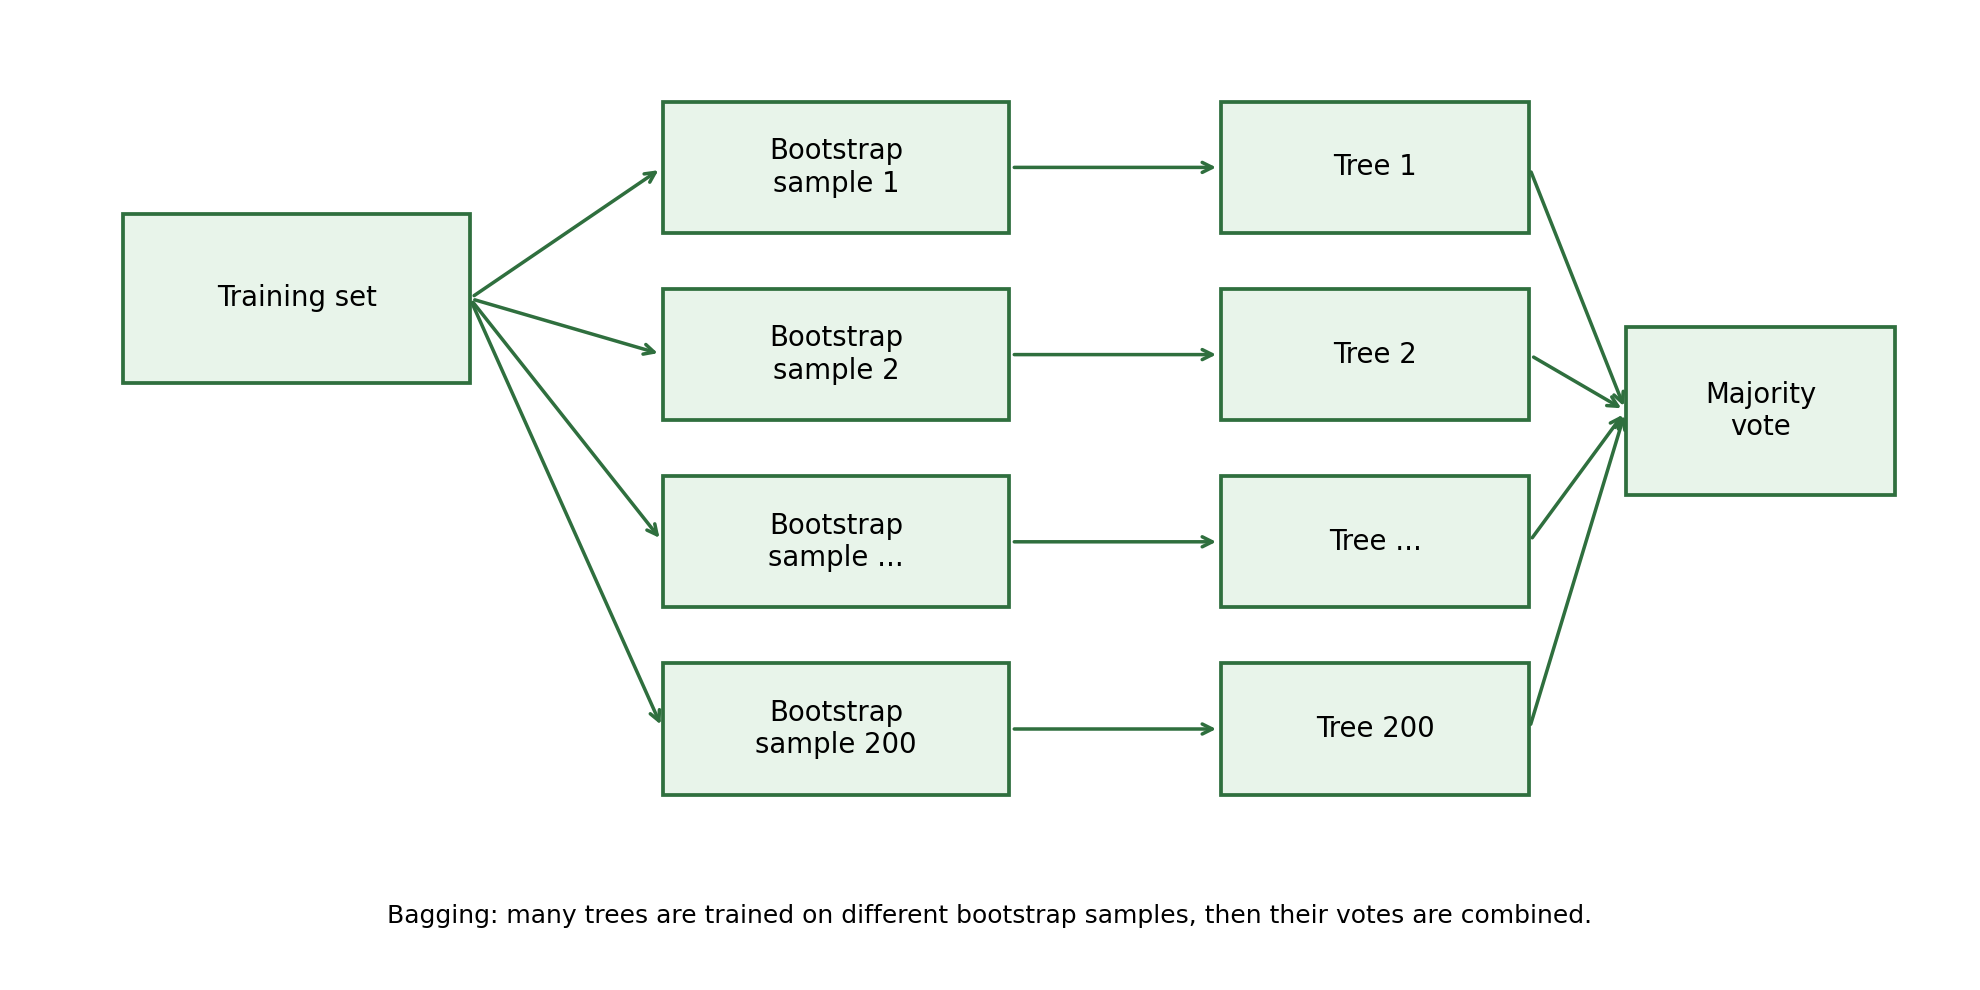
\includegraphics[width=0.92\textwidth]{q2_bagging_concept.png}
\caption{Η βασική ιδέα του Bagging: πολλά bootstrap δείγματα, πολλά δέντρα, μία τελική ψηφοφορία.}
\end{figure}

\subsection{Γιατί το Bagging συνήθως βοηθάει}

Το Bagging βοηθά κυρίως επειδή μειώνει τη διακύμανση του μοντέλου. Ένα δέντρο
μπορεί να είναι ασταθές, αλλά ο μέσος όρος ή η ψηφοφορία πολλών δέντρων είναι
συνήθως πιο σταθερή.

Στα δέντρα ταξινόμησης αυτό είναι ιδιαίτερα χρήσιμο, επειδή τα δέντρα μπορούν
να αλλάξουν αρκετά αν αλλάξει λίγο το training set. Με το Bagging, δεν
εμπιστευόμαστε μόνο ένα δέντρο, αλλά συνδυάζουμε πολλά.

%=============================================================================
\section{Πώς λύσαμε το ερώτημα βήμα-βήμα}
%=============================================================================

\subsection{Βήμα 1: Φορτώσαμε τα δεδομένα}

Όπως και στο πρώτο ερώτημα, ξεκινήσαμε διαβάζοντας το αρχείο CSV:

\begin{lstlisting}[language=Python]
df = pd.read_csv("../../Third Assigment/Data Analysis_2026 3rd Case_Data.csv")
\end{lstlisting}

Ο πίνακας \code{df} περιέχει όλες τις παρατηρήσεις και όλες τις μεταβλητές.

\subsection{Βήμα 2: Ορίσαμε predictors και target}

Κρατήσαμε ως predictors όλες τις μεταβλητές εκτός από τη \code{quality} και τη
\code{wine\_type}:

\begin{lstlisting}[language=Python]
features = [col for col in df.columns if col not in ("quality", "wine_type")]
X = df[features]
\end{lstlisting}

Έπειτα ορίσαμε τη μεταβλητή στόχο:

\begin{lstlisting}[language=Python]
y = (df["wine_type"] == "white").astype(int)
\end{lstlisting}

Άρα:

\begin{itemize}[nosep]
    \item \code{red} αντιστοιχεί σε 0,
    \item \code{white} αντιστοιχεί σε 1.
\end{itemize}

\subsection{Βήμα 3: Χωρίσαμε τα δεδομένα σε training και test}

Ο διαχωρισμός έγινε με:

\begin{lstlisting}[language=Python]
X_train, X_test, y_train, y_test = train_test_split(
    X,
    y,
    test_size=0.30,
    random_state=6931,
    stratify=y,
)
\end{lstlisting}

Αυτό σημαίνει ότι το μοντέλο εκπαιδεύτηκε σε 3706 παρατηρήσεις και
αξιολογήθηκε σε 1589 παρατηρήσεις που δεν είχε δει κατά την εκπαίδευση.

\subsection{Βήμα 4: Δημιουργήσαμε το Bagging μοντέλο}

Το μοντέλο δημιουργήθηκε ως εξής:

\begin{lstlisting}[language=Python]
model = BaggingClassifier(
    estimator=DecisionTreeClassifier(random_state=6931),
    n_estimators=200,
    random_state=6931,
    n_jobs=-1,
)
\end{lstlisting}

Ας εξηγήσουμε κάθε κομμάτι:

\begin{itemize}
    \item \code{BaggingClassifier}: δηλώνει ότι θα χρησιμοποιήσουμε τη μέθοδο
    Bagging για ταξινόμηση.
    \item \code{estimator=DecisionTreeClassifier(...)}: δηλώνει ότι το κάθε
    επιμέρους μοντέλο θα είναι δέντρο ταξινόμησης.
    \item \code{n\_estimators=200}: δηλώνει ότι θα εκπαιδευτούν 200 δέντρα.
    \item \code{random\_state=6931}: κάνει τη διαδικασία αναπαραγώγιμη.
    \item \code{n\_jobs=-1}: επιτρέπει στον υπολογιστή να χρησιμοποιήσει όλους
    τους διαθέσιμους πυρήνες για πιο γρήγορη εκπαίδευση.
\end{itemize}

\subsection{Βήμα 5: Εκπαιδεύσαμε το μοντέλο}

Η εκπαίδευση έγινε με:

\begin{lstlisting}[language=Python]
model.fit(X_train, y_train)
\end{lstlisting}

Στο σημείο αυτό το Bagging φτιάχνει 200 bootstrap δείγματα και εκπαιδεύει ένα
δέντρο σε κάθε δείγμα.

\subsection{Βήμα 6: Κάναμε προβλέψεις στο test set}

Μετά την εκπαίδευση, ζητήσαμε από το μοντέλο να προβλέψει τον τύπο κρασιού
για τις παρατηρήσεις του test set:

\begin{lstlisting}[language=Python]
y_pred = model.predict(X_test)
\end{lstlisting}

Η μεταβλητή \code{y\_pred} περιέχει τις προβλέψεις του Bagging.

\subsection{Βήμα 7: Υπολογίσαμε accuracy και test error}

Η ακρίβεια και το σφάλμα υπολογίστηκαν με:

\begin{lstlisting}[language=Python]
accuracy = accuracy_score(y_test, y_pred)
test_error = 1 - accuracy
\end{lstlisting}

Το \code{accuracy} είναι το ποσοστό σωστών προβλέψεων. Το \code{test\_error}
είναι το ποσοστό λανθασμένων προβλέψεων.

%=============================================================================
\section{Αποτελέσματα του Bagging}
%=============================================================================

Τα αποτελέσματα του Bagging με 200 εκτιμητές ήταν:

\begin{table}[H]
\centering
\caption{Βασικά αποτελέσματα Bagging.}
\begin{tabular}{lr}
\toprule
\textbf{Μέγεθος / μέτρο} & \textbf{Τιμή} \\
\midrule
Μοντέλο & Bagging \\
Πλήθος εκτιμητών & 200 \\
Random state & 6931 \\
Πλήθος predictors & 11 \\
Πλήθος test παρατηρήσεων & 1589 \\
Test accuracy & 0.9660 \\
Test error & 0.0340 \\
\bottomrule
\end{tabular}
\end{table}

Η τιμή:

\begin{center}
\textbf{Test accuracy = 0.9660}
\end{center}

σημαίνει ότι το μοντέλο ταξινόμησε σωστά περίπου το 96.60\% των test
παρατηρήσεων.

Αντίστοιχα:

\begin{center}
\textbf{Test error = 0.0340}
\end{center}

σημαίνει ότι έκανε λάθος περίπου στο 3.40\% των test παρατηρήσεων.

\subsection{Confusion matrix}

Ο confusion matrix του Bagging ήταν:

\begin{table}[H]
\centering
\caption{Confusion matrix για το Bagging.}
\begin{tabular}{lcc}
\toprule
& \textbf{Πρόβλεψη: red} & \textbf{Πρόβλεψη: white} \\
\midrule
\textbf{Πραγματικό: red} & 365 & 26 \\
\textbf{Πραγματικό: white} & 28 & 1170 \\
\bottomrule
\end{tabular}
\end{table}

\begin{figure}[H]
\centering
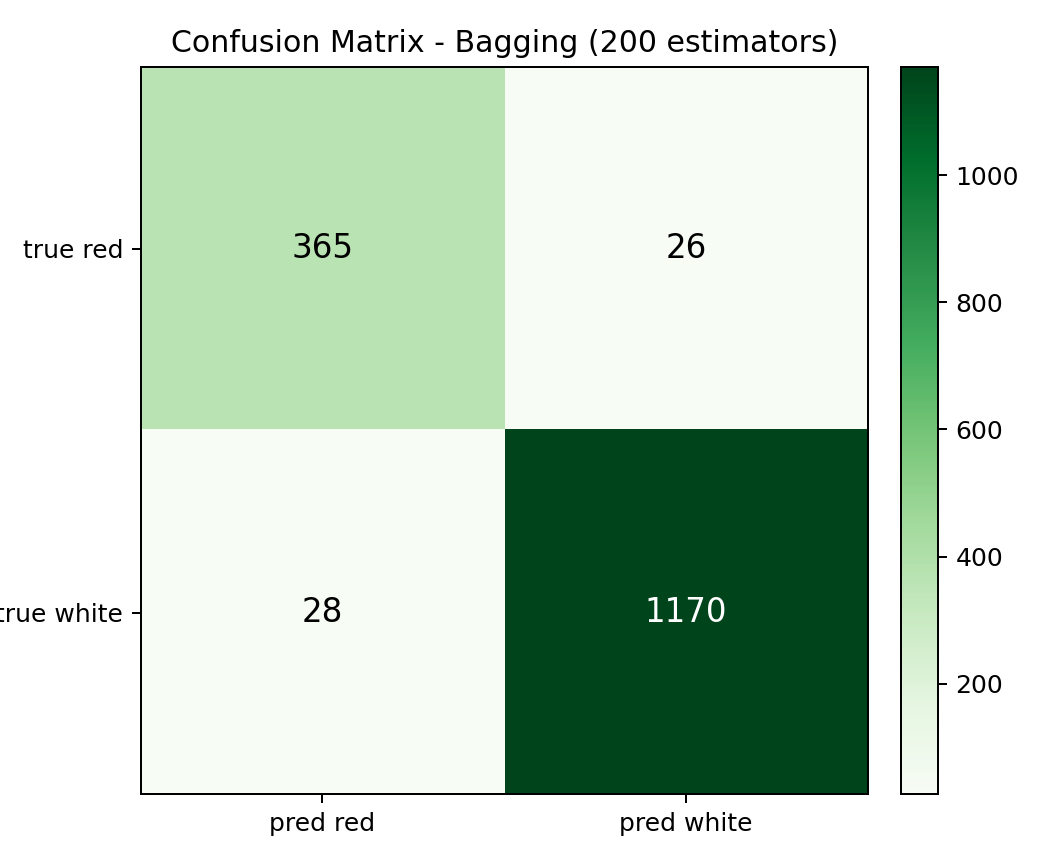
\includegraphics[width=0.62\textwidth]{q2_confusion_matrix.png}
\caption{Γραφική απεικόνιση του confusion matrix για το Bagging.}
\end{figure}

\subsection{Πώς διαβάζουμε τα αποτελέσματα}

Ο confusion matrix μάς λέει τα εξής:

\begin{itemize}
    \item 365 κόκκινα κρασιά ταξινομήθηκαν σωστά ως κόκκινα.
    \item 26 κόκκινα κρασιά ταξινομήθηκαν λάθος ως λευκά.
    \item 28 λευκά κρασιά ταξινομήθηκαν λάθος ως κόκκινα.
    \item 1170 λευκά κρασιά ταξινομήθηκαν σωστά ως λευκά.
\end{itemize}

Άρα οι σωστές προβλέψεις είναι:

\[
    365 + 1170 = 1535.
\]

Οι συνολικές test παρατηρήσεις είναι:

\[
    365 + 26 + 28 + 1170 = 1589.
\]

Επομένως:

\[
    \text{Accuracy} = \frac{1535}{1589} = 0.9660.
\]

Τα συνολικά λάθη είναι:

\[
    26 + 28 = 54.
\]

Άρα:

\[
    \text{Test Error} = \frac{54}{1589} = 0.0340.
\]

%=============================================================================
\section{Σύγκριση με το απλό δέντρο του Ερωτήματος 1}
%=============================================================================

Είναι χρήσιμο να συγκρίνουμε το Bagging με το απλό δέντρο ταξινόμησης του
πρώτου ερωτήματος. Στο πρώτο ερώτημα είχαμε μόνο ένα δέντρο με
\code{max\_depth=2}. Στο δεύτερο ερώτημα έχουμε 200 δέντρα, τα οποία
συνδυάζονται με ψηφοφορία.

\begin{table}[H]
\centering
\caption{Σύγκριση απλού δέντρου και Bagging.}
\begin{tabular}{lrr}
\toprule
\textbf{Μοντέλο} & \textbf{Test Accuracy} & \textbf{Test Error} \\
\midrule
Decision Tree (\code{max\_depth=2}) & 0.9339 & 0.0661 \\
Bagging (200 estimators) & 0.9660 & 0.0340 \\
\bottomrule
\end{tabular}
\end{table}

Η ακρίβεια αυξήθηκε από 0.9339 σε 0.9660. Η βελτίωση είναι:

\[
    0.9660 - 0.9339 = 0.0321.
\]

Δηλαδή το Bagging αύξησε την ακρίβεια κατά περίπου 3.21 ποσοστιαίες μονάδες.

Αντίστοιχα, τα λάθη μειώθηκαν:

\begin{center}
\begin{tabular}{lrr}
\toprule
\textbf{Μοντέλο} & \textbf{Λάθη στο test set} & \textbf{Σωστές προβλέψεις} \\
\midrule
Decision Tree & 105 & 1484 \\
Bagging & 54 & 1535 \\
\bottomrule
\end{tabular}
\end{center}

Άρα το Bagging έκανε:

\[
    105 - 54 = 51
\]

λιγότερα λάθη από το απλό δέντρο του πρώτου ερωτήματος.

\subsection{Γιατί βελτιώθηκε η απόδοση}

Η βελτίωση είναι αναμενόμενη. Το απλό δέντρο του πρώτου ερωτήματος ήταν πολύ
περιορισμένο, επειδή είχε μέγιστο βάθος 2. Αντίθετα, το Bagging χρησιμοποιεί
πολλά δέντρα και συνδυάζει τις αποφάσεις τους.

Αν κάποιο δέντρο κάνει λάθος σε μία παρατήρηση, αυτό δεν σημαίνει απαραίτητα
ότι θα κάνει λάθος και το συνολικό Bagging μοντέλο. Η τελική απόφαση
λαμβάνεται από την πλειοψηφία των δέντρων. Έτσι, τα μεμονωμένα λάθη μπορούν να
αντισταθμιστούν.

%=============================================================================
\section{Ποια χαρακτηριστικά χρησιμοποίησε περισσότερο το Bagging}
%=============================================================================

Αν και το Bagging αποτελείται από πολλά δέντρα και είναι λιγότερο απλό από ένα
μόνο δέντρο, μπορούμε να πάρουμε μία ένδειξη για το ποιες μεταβλητές ήταν πιο
σημαντικές. Αυτό έγινε υπολογίζοντας τη μέση σημαντικότητα κάθε μεταβλητής στα
200 δέντρα.

\begin{figure}[H]
\centering
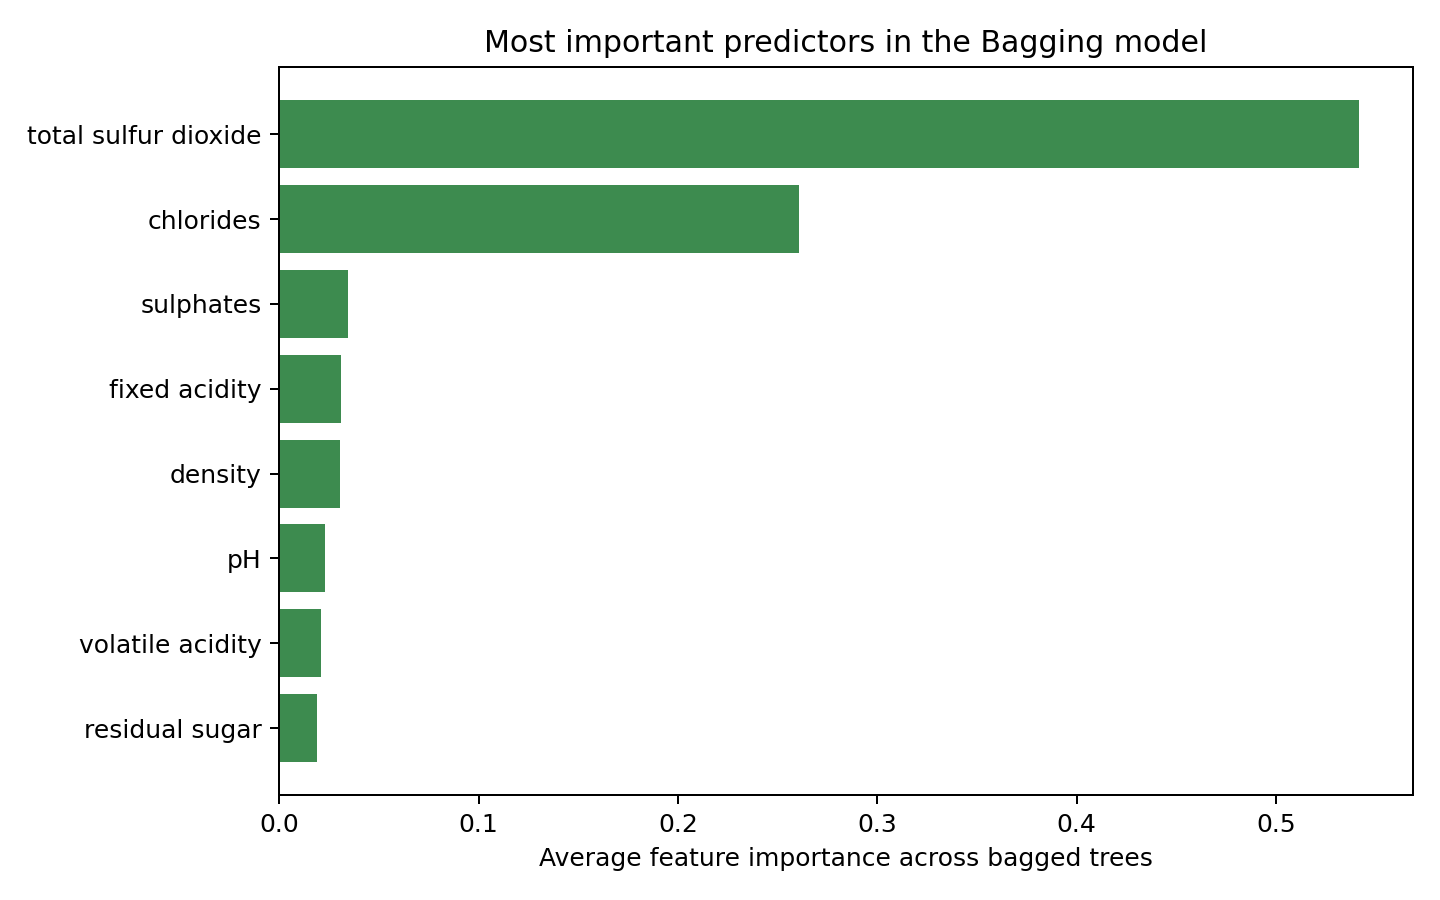
\includegraphics[width=0.82\textwidth]{q2_bagging_feature_importance.png}
\caption{Οι σημαντικότερες μεταβλητές στο Bagging μοντέλο.}
\end{figure}

\begin{table}[H]
\centering
\caption{Μέση σημαντικότητα χαρακτηριστικών στο Bagging.}
\small
\begin{tabular}{lr}
\toprule
\textbf{Μεταβλητή} & \textbf{Σημαντικότητα} \\
\midrule
\code{total sulfur dioxide} & 0.5416 \\
\code{chlorides} & 0.2609 \\
\code{sulphates} & 0.0347 \\
\code{fixed acidity} & 0.0312 \\
\code{density} & 0.0303 \\
\code{pH} & 0.0228 \\
\code{volatile acidity} & 0.0211 \\
\code{residual sugar} & 0.0187 \\
\code{citric acid} & 0.0139 \\
\code{alcohol} & 0.0135 \\
\code{free sulfur dioxide} & 0.0112 \\
\bottomrule
\end{tabular}
\end{table}

Παρατηρούμε ότι οι δύο πιο σημαντικές μεταβλητές είναι:

\begin{itemize}
    \item \code{total sulfur dioxide}
    \item \code{chlorides}
\end{itemize}

Αυτό είναι ενδιαφέρον, γιατί και στο απλό δέντρο του πρώτου ερωτήματος αυτές
οι μεταβλητές ήταν οι βασικές μεταβλητές που χρησιμοποιήθηκαν στους κανόνες
απόφασης. Άρα υπάρχει συνέπεια ανάμεσα στο απλό δέντρο και στο Bagging: και
τα δύο μοντέλα θεωρούν πολύ χρήσιμες τις μεταβλητές που σχετίζονται με τα
θειώδη και τα χλωριούχα άλατα.

%=============================================================================
\section{Τελικός σχολιασμός για το Ερώτημα 2}
%=============================================================================

Η μέθοδος Bagging με 200 εκτιμητές πέτυχε πολύ υψηλή απόδοση στην πρόβλεψη του
τύπου κρασιού. Η test accuracy ήταν 0.9660, δηλαδή το μοντέλο ταξινόμησε σωστά
περίπου το 96.60\% των test παρατηρήσεων.

Σε σχέση με το απλό δέντρο του πρώτου ερωτήματος, το Bagging είχε σαφώς
καλύτερη απόδοση. Το απλό δέντρο έκανε 105 λάθη στο test set, ενώ το Bagging
έκανε 54 λάθη. Επομένως, το Bagging μείωσε τα λάθη κατά 51 παρατηρήσεις.

Η βελτίωση αυτή οφείλεται στη βασική ιδέα του Bagging: αντί να βασιστούμε σε
ένα μόνο δέντρο, εκπαιδεύουμε πολλά δέντρα σε διαφορετικά bootstrap δείγματα
και συνδυάζουμε τις προβλέψεις τους. Με αυτόν τον τρόπο μειώνεται η αστάθεια
ενός μεμονωμένου δέντρου και προκύπτει ένα πιο αξιόπιστο μοντέλο.

\subsection{Σύντομη απάντηση που μπορεί να μπει στην εργασία}

Για το δεύτερο ερώτημα εφαρμόστηκε η μέθοδος Bagging με
\code{n\_estimators=200}. Ως βασικός εκτιμητής χρησιμοποιήθηκε δέντρο
ταξινόμησης, ενώ οι προβλεπτικές μεταβλητές ήταν όλες οι διαθέσιμες μεταβλητές
εκτός από τη \code{quality}. Ο διαχωρισμός των δεδομένων έγινε σε training set
70\% και test set 30\% με \code{random\_state=6931}. Το μοντέλο πέτυχε test
accuracy 0.9660 και test error 0.0340. Ο confusion matrix έδειξε ότι
ταξινομήθηκαν σωστά 365 κόκκινα και 1170 λευκά κρασιά, ενώ έγιναν συνολικά 54
λάθη. Σε σύγκριση με το απλό δέντρο ταξινόμησης του πρώτου ερωτήματος, το
Bagging παρουσίασε σημαντική βελτίωση, καθώς μείωσε τα λάθη από 105 σε 54.

%=============================================================================
\appendix
\section{Αρχεία που δημιουργήθηκαν για το report}
%=============================================================================

Για το επεξηγηματικό report του Ερωτήματος 2 δημιουργήθηκαν τα παρακάτω
αρχεία:

\begin{itemize}
    \item \code{q2\_explanatory\_bagging.py}: script που αναπαράγει τη λύση.
    \item \code{q2\_explanatory\_results.csv}: συγκεντρωτικός πίνακας
    αποτελεσμάτων.
    \item \code{q2\_vs\_q1\_comparison.csv}: σύγκριση Bagging με το δέντρο του
    Ερωτήματος 1.
    \item \code{q2\_confusion\_matrix.png}: εικόνα του confusion matrix.
    \item \code{q2\_bagging\_concept.png}: απλό σχήμα που εξηγεί τη μέθοδο
    Bagging.
    \item \code{q2\_bagging\_feature\_importance.csv}: μέση σημαντικότητα
    χαρακτηριστικών.
    \item \code{q2\_bagging\_feature\_importance.png}: γράφημα σημαντικότητας
    χαρακτηριστικών.
    \item \code{explanatory\_report\_q2\_bagging.tex}: το παρόν LaTeX αρχείο.
\end{itemize}

\end{document}
